%
% Complete documentation on the extended LaTeX markup used for Insight
% documentation is available in ``Documenting Insight'', which is part
% of the standard documentation for Insight.  It may be found online
% at:
%
%     http://www.itk.org/

\documentclass{InsightArticle}

\usepackage[dvips]{graphicx}
\usepackage{float}
\usepackage{subfigure}
\usepackage{amsmath} % for cases{}
\usepackage{graphicx}

%%%%%%%%%%%%%%%%%%%%%%%%%%%%%%%%%%%%%%%%%%%%%%%%%%%%%%%%%%%%%%%%%%
%
%  hyperref should be the last package to be loaded.
%
%%%%%%%%%%%%%%%%%%%%%%%%%%%%%%%%%%%%%%%%%%%%%%%%%%%%%%%%%%%%%%%%%%
\usepackage[dvips,
bookmarks,
bookmarksopen,
backref,
colorlinks,linkcolor={blue},citecolor={blue},urlcolor={blue},
]{hyperref}


\title{Poisson Hole Filling in ITK and VNL}

% 
% NOTE: This is the last number of the "handle" URL that 
% The Insight Journal assigns to your paper as part of the
% submission process. Please replace the number "1338" with
% the actual handle number that you get assigned.
%
\newcommand{\IJhandlerIDnumber}{3253}

% Increment the release number whenever significant changes are made.
% The author and/or editor can define 'significant' however they like.
\release{0.00}

% At minimum, give your name and an email address.  You can include a
% snail-mail address if you like.

\author{David Doria}
\authoraddress{Rensselaer Polytechnic Institute, Troy NY}


\begin{document}

%
% Add hyperlink to the web location and license of the paper.
% The argument of this command is the handler identifier given
% by the Insight Journal to this paper.
% 
\IJhandlefooter{\IJhandlerIDnumber}


\ifpdf
\else
   %
   % Commands for including Graphics when using latex
   % 
   \DeclareGraphicsExtensions{.eps,.jpg,.gif,.tiff,.bmp,.png}
   \DeclareGraphicsRule{.jpg}{eps}{.jpg.bb}{`convert #1 eps:-}
   \DeclareGraphicsRule{.gif}{eps}{.gif.bb}{`convert #1 eps:-}
   \DeclareGraphicsRule{.tiff}{eps}{.tiff.bb}{`convert #1 eps:-}
   \DeclareGraphicsRule{.bmp}{eps}{.bmp.bb}{`convert #1 eps:-}
   \DeclareGraphicsRule{.png}{eps}{.png.bb}{`convert #1 eps:-}
\fi


\maketitle


\ifhtml
\chapter*{Front Matter\label{front}}
\fi


% The abstract should be a paragraph or two long, and describe the
% scope of the document.
\begin{abstract}
\noindent
This code provides an implementation of two techniques from ``Poisson Image Editing'' on ITK images. First, we fill a hole in an image given only the pixel values on the boundary. Second, we copy a patch of an image into another image and make the result as smooth as possible.

\end{abstract}

\IJhandlenote{\IJhandlerIDnumber}

\tableofcontents

%%%%%%%%%%%%%%%%%
\section{Introduction}
This code provides an implementation of two techniques from ``Poisson Image Editing'' (\cite{PoissonImageEditing}) on ITK images. First, we fill a hole in an image given only the pixel values on the boundary. Second, we copy a patch of an image into another image and make the result as smooth as possible.

%%%%%%%%%%%%%%%%%
\section{Hole Filling}
The idea here is to fill in a missing region in an image in a plausible way. This is best motivated with an example. In Figure \ref{fig:HoleFilling}, the goal is to remove the plane from the image in Figure \ref{fig:HoleFilling:original}. To do this, we simply specify the region to be removed (shown in Figure \ref{fig:HoleFilling:mask}). The result of the filling is shown in Figure \ref{fig:HoleFilling:filled}.

\begin{figure}[H]
\centering
\subfigure[Original image]{
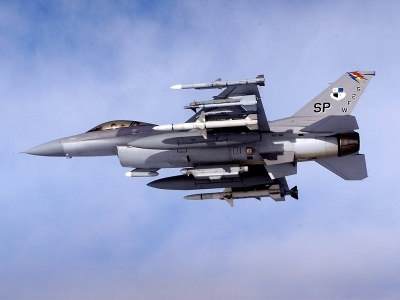
\includegraphics[width=0.3\linewidth]{images/plane}
\label{fig:HoleFilling:original}
}
\subfigure[Mask]{
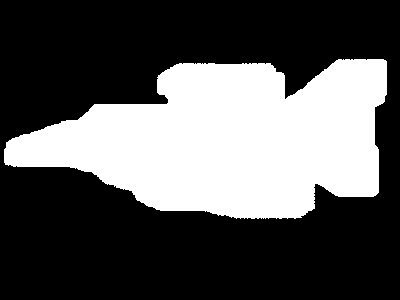
\includegraphics[width=0.3\linewidth]{images/planeMask}
\label{fig:HoleFilling:mask}
}
\subfigure[Filled image]{

\includegraphics[width=0.3\linewidth]{images/planeFilled}
\label{fig:HoleFilling:filled}
}
\caption{A demonstration of Poisson hole filling}
\label{fig:HoleFilling}
\end{figure}

\subsection{Input}
The inputs to this class are:
\begin{itemize}
\item An image, $I$.
\item A mask. Non-zero pixels indicate the region to fill. The mask must be the same size as the image, and must not have non-zero pixels on its border.
\end{itemize}

\subsection{Concept}
It has been shown using Calculus of Variations that the best solution for the region inside the hole, $H$, is given by the solution to 

\begin{equation}
\nabla^2 H = 0
\end{equation}

while ensuring $H=I$ on the boundary of the hole. This setup is a Laplace equation with Dirchlet (aka ``first order) boundary conditions. 

\subsection{Discrete Solution}
The Laplace operator is given by
\begin{equation}
 \nabla^2 f = \sum_{i=1}^n \frac{\partial^2 f}{\partial x_i^2}
\end{equation}

A discrete approximation to this function at a pixel $(x,y)$ is given by
\begin{equation}
 \nabla^2 f(x,y) = f(x-1,y) + f(x+1,y) + f(x,y-1) + f(x,y+1) - 4f(x,y)
\end{equation}

Another way to write this is to multiply the pixel and its neighbors by a kernel:
\begin{equation}
\begin{pmatrix}
0 & 1 & 0 \\
1 & -4 & 1\\
0 & 1 & 0
\end{pmatrix}
\end{equation}


From this, for each unknown pixel $u_{i,j}$, the equation is:

\begin{equation}
\label{eqn:DiscreteLaplacian}
4 u_{i,j} - u_{i+1,j} - u_{i-1,j} - u_{i,j+1} - u_{i,j-1} = 0
\end{equation}

To solve the Laplace equation over the entire image, we can write a linear system of equations. We create a variable for every component of every pixel to be filled. That is, if there are $N$ pixels to be filled and each pixel consists of $C$ components (i.e. 3 in the case of an RGB image), there are $NC$ variables in the linear system. 

A sparse matrix $U$ is constructed row by row, one row per variable. In each row, a $4$ is placed in the column corresponding to the variable id. A $-1$ is placed in the column corresponding to the variable id of any non-border 4-connected neighbor.

When one of the pixels appearing in equation \ref{eqn:DiscreteLaplacian} is on the border of the hole (and is therefore known), $u_{.,.}$ is replaced with $p_{.,.}$, the value of the pixel from the original image. In this case, a $-1$ is not placed in the $U$ matrix, but instead the value is moved to the right side of the equation to construct the $b$ vector, the right hand side of the linear system equation.

A vector $H_v$, the vectorized version of the solution to the set of hole pixels, of length $NC$ is created as the unknown vector to be solved in a system of equations.

The linear system is then
\begin{equation}
 U^T H_v = b
\end{equation}

is then solved for $H_v$. The resulting $H_v$ is then remapped back to the pixels corresponding to each variable id to construct $H$.

\subsection{Code Snippet}

Using this class is very straight forward, as shown below:

\begin{verbatim}
  PoissonEditing poissonEditing;
  poissonEditing.SetImage(imageReader->GetOutput());
  poissonEditing.SetMask(maskReader->GetOutput());
  poissonEditing.FillRegion(outputImage);

  Helpers::ClampImage<FloatVectorImageType>(outputImage);
  Helpers::CastAndWriteImage<FloatVectorImageType>(outputImage, "output.png");
\end{verbatim}


%%%%%%%%%%%%%%%%%
\section{Region Copying}
In the problem of region copying (aka seamless cloning), we are interested in copying a region from one image into another image in a visually pleasing way. This is again best motivated with an example. In Figure \ref{fig:RegionCopying}, the goal is to copy the plane from the image with the sky background into the image of the canyon. 

\begin{figure}[H]
\centering
\subfigure[Original image]{
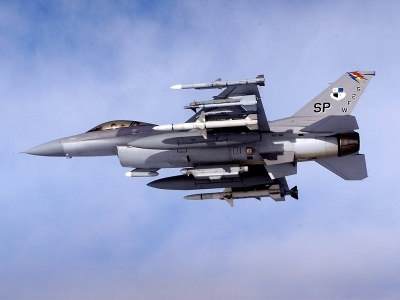
\includegraphics[width=0.2\linewidth]{images/plane}
\label{fig:RegionCopying:original}
}
\subfigure[Mask]{
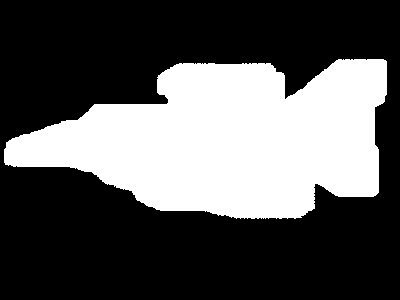
\includegraphics[width=0.2\linewidth]{images/planeMask}
\label{fig:RegionCopying:mask}
}
\subfigure[Target Image]{
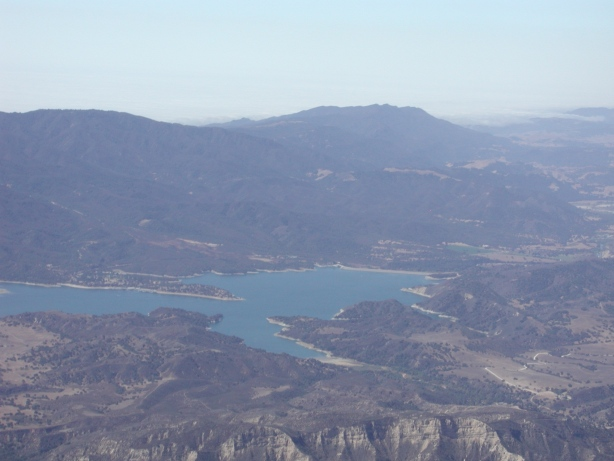
\includegraphics[width=0.2\linewidth]{images/planeTarget}
\label{fig:RegionCopying:target}
}
\subfigure[Resulting Image]{
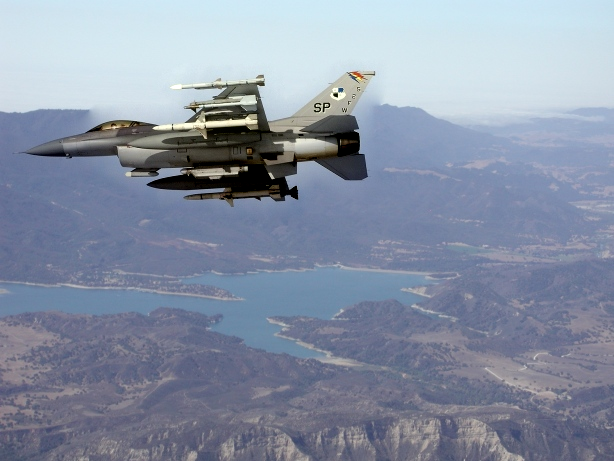
\includegraphics[width=0.2\linewidth]{images/planeCopyingResult}
\label{fig:RegionCopying:target}
}
\caption{A demonstration of Poisson region copying}
\label{fig:RegionCopying}
\end{figure}

\subsection{Input}
The inputs to this class are:
\begin{itemize}
\item A source image, $S$.
\item A target image, $T$.
\item A mask, $M$. Non-zero pixels indicate the region to fill. The mask must be the same size as the image, and must not have non-zero pixels on its border.
\end{itemize}

\subsection{Concept}

In \cite{PoissonImageEditing}, it was argued that a good way to copy a region of one image into another image is to do something very similar to hole filling, but additionally introduce a ''guidance field``, $G$. That is, the way to copy a region of one image into another is to solve the equation

\begin{equation}
\nabla^2 H = div(G)
\end{equation}

The boundary condition this time is again first order and specifies that the resulting $H$ be equal to the target image, $T$, at the hole boundary.

The suggested guidance field $G$ is the gradient of the source image. That is,

\begin{equation}
G = \nabla S
\end{equation}

In this case, the right hand side of the equation has become $div(\nabla S)$, which is exactly the Laplacian of $S$.

\subsection{Discrete Solution}
Just as before, the discrete Laplacian equation is written for each pixel, but this time the right hand side is set to $\nabla^2 S(i,j)$.
\begin{equation}
\label{eqn:DiscreteLaplacian}
4 u_{i,j} - u_{i+1,j} - u_{i-1,j} - u_{i,j+1} - u_{i,j-1} = \nabla^2 S(i,j)
\end{equation}

The linear system 
\begin{equation}
 U^T H_v = b
\end{equation}

is created and solved identically as before.

\subsection{Code Snippet}

Using this class is very straight forward, as shown below:

\begin{verbatim}
  PoissonCloning<FloatVectorImageType> poissonCloning;
  poissonCloning.SetSourceImage(sourceImageReader->GetOutput());
  poissonCloning.SetTargetImage(targetImageReader->GetOutput());
  poissonCloning.SetMask(maskReader->GetOutput());
  poissonCloning.PasteMaskedRegionIntoTargetImage(outputImage);

  Helpers::ClampImage<FloatVectorImageType>(outputImage);
  Helpers::CastAndWriteImage<FloatVectorImageType>(outputImage, "output.png");
\end{verbatim}

%%%%%%%%%%%%
\section{Reconstructing an Image from Its Derivatives}
For this task, we can use a very similar method. This time, There are two equations to be solved simultaneously:
\begin{equation}
\frac{d}{dx}(U) = D_x
\end{equation}
\begin{equation}
\frac{d}{dy}(U) = D_y
\end{equation}

$D_x$ and $D_y$ are the known derivative images.

We can construct the same type of linear system to solve for the components of $U$ that best satisfy both equations. We use the Sobel operators

\begin{equation}
S_x =
\begin{pmatrix}
-1 & 0 & 1 \\
-2 & 0 & 2\\
-1 & 0 & 1
\end{pmatrix}
\end{equation}

and

\begin{equation}
S_x =
\begin{pmatrix}
-1 & -2 & -1 \\
0 & 0 & 0\\
1 & 2 & 1
\end{pmatrix}
\end{equation}

By applying these operators to every pixel in the unknown image $U$, we can write a system of equations, two for each pixel:
\begin{equation}
- u_{i-1,j-1} -2 u_{i-1,j} - u_{i-1,j+1} + u_{i+1,j+1} + 2 u_{i+1,j} + u_{i,j+1} = D_x(i,j)
\end{equation}

\begin{equation}
- u_{i-1,j-1} -2 u_{i,j-1} - u_{i+1,j+1} + u_{i-1,j-1} + 2 u_{i,j+1} + u_{i+1,j+1} = D_y(i,j)
\end{equation}

Again, we simply place the coefficient of each term in the column of the matrix corresponding the variable id of the pixel. As usual, we move the term to the right side of the equation (to contribute to the $b$ vector) if the pixel is known.

\begin{figure}[H]
\centering
\subfigure[Original image]{

\includegraphics[width=0.2\linewidth]{images/smiley}
\label{fig:RegionCopying:original}
}
\subfigure[$D_x$]{

\includegraphics[width=0.2\linewidth]{images/smileyXDerivative}
\label{fig:RegionCopying:mask}
}
\subfigure[$D_y$]{

\includegraphics[width=0.2\linewidth]{images/smileyYDerivative}
\label{fig:RegionCopying:target}
}
\subfigure[Resulting Image]{

\includegraphics[width=0.2\linewidth]{images/smileyReconstructed}
\label{fig:RegionCopying:target}
}
\caption{A demonstration of reconstructing an image from its derivatives}
\label{fig:RegionCopying}
\end{figure}

%%%%%%%%%%%%
\section{Notes}
\subsection{Clamping outputs}
It is important to note that in both problems, the linear system is solved in a least squared sense with no constraints. This allows the resulting image to take invalid values (i.e. greater than 255 or less than 0). The resulting images must therefore be clamped or scaled to ensure the output has an appropriate range.

\subsection{Efficiency}
The examples in this document took about 2 minutes to complete on a single core machine.

\bibliography{InsightJournal}
\bibliographystyle{plain} % MUST include this line or will get ``undefined reference'' errors

\end{document}

